\documentclass[11pt,a4paper]{ctexart}
\usepackage[margin=2.35cm]{geometry}
\usepackage{amsmath,booktabs,graphicx,float,caption,xcolor,needspace}
\usepackage[colorlinks=true,urlcolor=blue!55!black,linkcolor=blue!55!black]{hyperref}
\graphicspath{{figures/}}
\captionsetup{font=small,labelfont=bf}
\setlength{\parskip}{0.35em}
\renewcommand{\arraystretch}{1.18}
\newcommand{\Efixed}{E_{\mathrm{fixed}}}
\title{\textbf{鲁棒却不可判别}\\[4pt]
\large 单次抓取下的科大网站群结构韧性与失效聚集}
\author{复杂系统分析课程大作业小组}
\date{}

\begin{document}
\maketitle

\begin{abstract}
本文以中国科学技术大学网站群的一次超链接抓取为样本，研究两件事。第一，观测网络在随机和定向移除下有多耐受。第二，出链缺失使哪些失效问题无法回答。基于 674 个节点的无向主分量，随机移除的均值曲线在删去约 40.8\% 的节点后首次跌破原连通规模的 50\%，按介数排序移除时的比例为 11.28\%。移除 162 个标为全挂的站点后，固定分母效率为 0.2039，同数量均匀随机均值为 0.1610，按观测入度分层后的随机均值为 0.1876。分层后差距缩小约六成，方向在本次模拟中保持一致。由于这 162 个站点的出链均未采到，快照中的失效站点之间没有可见连边，真实站点失效是否相互聚集仍无法判别。

\noindent\textbf{关键词}\quad 超链接网络；结构韧性；抓取删失；固定分母效率
\end{abstract}

\section{研究问题}

校园网站之间的链接可用于研究组织内部的信息连接。本文借鉴复杂网络中随机故障与定向移除的比较方法\cite{albert2000}，并沿用有向网页网络的连通结构分析\cite{broder2000}。一次抓取同时记录了站点状态和能看到的链接，但状态本身也影响出链能否被采到。分析需要分别处理记录下来的网络结构和缺失的部分。本文以两个可核查的问题组织结果。

\begin{enumerate}
  \item 在同一张观测图上，随机与定向移除对连通性有多大影响？观测失效名单与随机名单的差异在匹配入度后有多大？
  \item 当失效站点的出链从抓取中缺失时，观测图可以回答哪些关于失效聚集和健康判别的问题？
\end{enumerate}

\section{数据与方法}

\subsection{图的表示与站点状态}

以子域为节点，以观测到的跨子域超链接为有向边。原料包含 671 个有属性站点、2,788 条有向链接和 8,115 条已收录的 URL 记录。把链接中出现的额外引用节点计入后，有向全图共有 676 个节点。A4 的有向结构结果使用全图。E3 和 E5 的韧性实验将链接无向化、二值化，取最大的连通分量作为基准图，共 674 个节点和 2,497 条边。

在 162 个标为全挂的子域中，按现有抓取记录和状态码规则，有 129 个归为真失效、32 个归为访问受限或跳过（实际可用性未确认）、1 个待定。两种名单在 E5 中分别使用。站点状态只对应这份快照及其分类口径。

\subsection{结构韧性与对照}

以移除比例 \(f=k/n_0\) 为横轴，用移除后最大连通分量的节点数与原始节点数之比 \(S(f)\) 衡量连通性。文中阈值定义为 \(S(f)\) 首次低于指定水平时的 \(f\)。随机策略的主结果先对每个 \(f\) 的曲线取平均，再找其首次跌破的位置。定向策略采用静态排序，按原图计算的中心性依次移除节点。

E5 用固定分母效率度量移除后的网络。令 \(d_k(i,j)\) 为移除名单后剩余图上的距离，则
\[
  \Efixed(k)=\frac{1}{n_0(n_0-1)}
  \sum_{\substack{i\ne j,\ i,j\text{ 均保留}\\ d_k(i,j)<\infty}}
    \frac{1}{d_k(i,j)} .
\]
本研究 \(n_0=674\)。被移除或变得不可达的节点对贡献为零。比较不同名单时采用同一个基准图和同一个 \(k\)。

补充实验把每个基准图节点按原有向图在同一节点集上的观测入度划入 \(0\)、\(1\)、\(2\)--\(3\)、\(4\)--\(7\)、\(8+\) 五层。每次从各层无放回抽取与观测名单相同的节点数。每种名单抽取 300 次，报告均值与第 2.5、97.5 百分位。分层约束的是观测入度的区间频数。

\section{结果}

\subsection{观测网络对不同移除策略的耐受性}

最大连通分量跌破原规模一半时，随机移除均值曲线对应 40.80\%（275 个节点），按介数排序为 11.28\%（76 个节点），按度排序为 11.42\%（77 个节点）。无权无向 PageRank 排序在该阈值上同为 11.28\%。用 25\% 作为阈值时，随机为 63.65\%，按介数为 17.51\%。两个阈值下均可见不同策略的差距。这些曲线刻画的是无向子域图上的结构情景。

\begin{figure}[H]
  \centering
  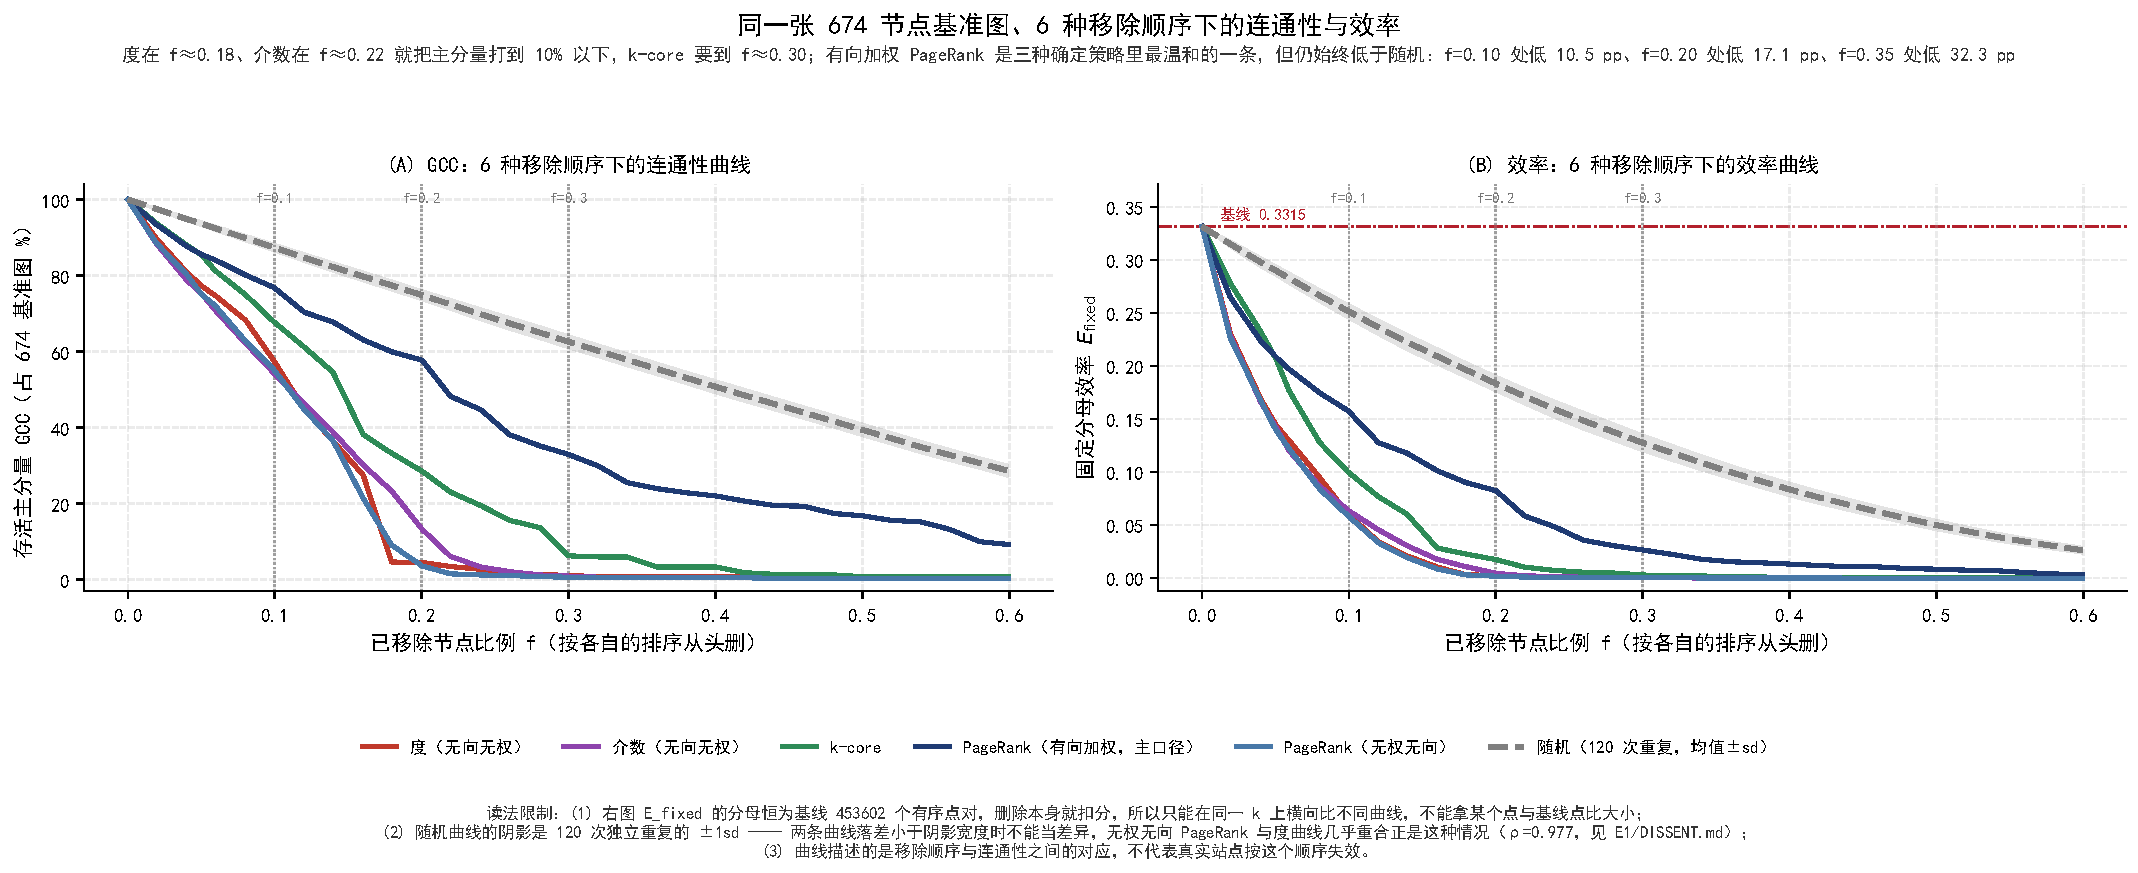
\includegraphics[width=0.95\linewidth]{fig06_attack_curves.pdf}
  \caption{不同移除策略下的结构韧性曲线。正文阈值取自 E3 的 674 节点静态实验，PageRank 指标以该实验标注的具体口径为准。}
\end{figure}

\Needspace{9\baselineskip}
\subsection{观测失效名单与两种随机对照}

在当前抓取图上，移除观测失效名单后保留的效率高于同数量均匀随机平均值。改用入度分层对照后，162 站点名单的差距从 0.0430 缩至 0.0163，129 站点名单的差距从 0.0371 缩至 0.0133，两者均缩小约六成。在这两组各 300 次抽样中，观测名单的剩余效率均高于分层随机抽样的所有取值。这是对基线选择的敏感性结果，适用于当前网络、名单和入度分层。

\begin{table}[H]
\centering
\caption{固定移除数量后的剩余效率}
\begin{tabular}{lrrrr}
\toprule
情景 & 数量 & 观测名单 & 均匀随机均值 & 入度分层随机均值 \\
\midrule
全挂标记 & 162 & 0.2039 & 0.1610 & 0.1876 \\
判为真失效 & 129 & 0.2280 & 0.1910 & 0.2147 \\
\bottomrule
\end{tabular}
\end{table}

\begin{figure}[H]
\centering
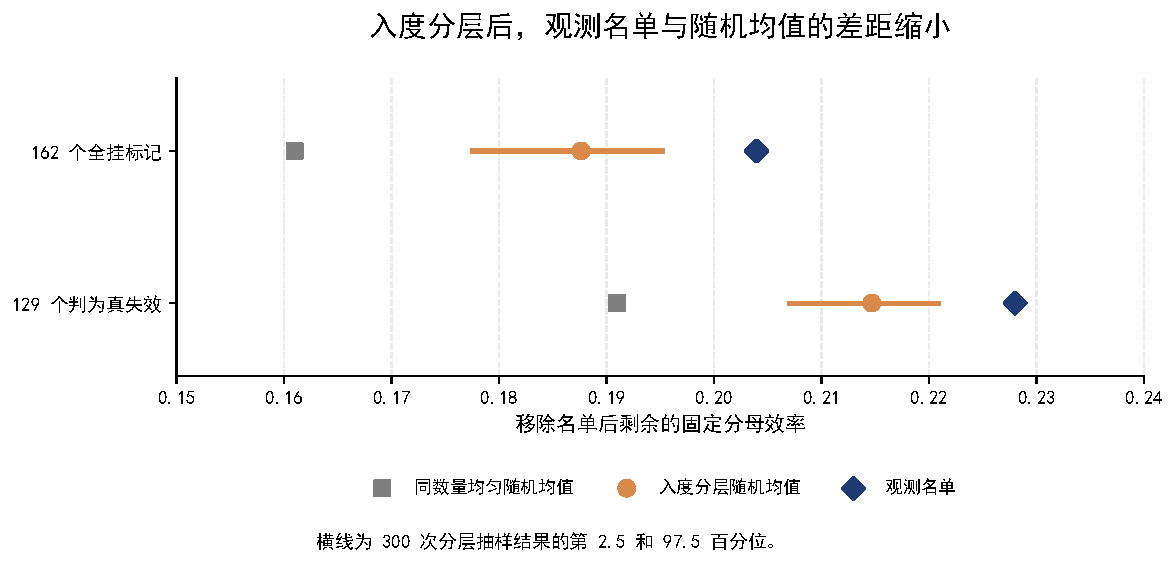
\includegraphics[width=0.95\linewidth]{fig12_matched_efficiency.pdf}
\caption{均匀随机基线与入度分层基线。横线表示分层抽样的经验区间。}
\end{figure}

\Needspace{9\baselineskip}
\subsection{失效聚集的观测边界}

162 个全挂站点的出链均未被采到。因此，从这些站点发出的失效站点之间的链接，在这份快照里不可见。图示中的两张可能原图具有不同的失效站点互连结构，按这个抓取规则却产生同一张观测图。真实网络中的失效聚集由此无法仅凭一次快照判别。

\begin{figure}[H]
\centering
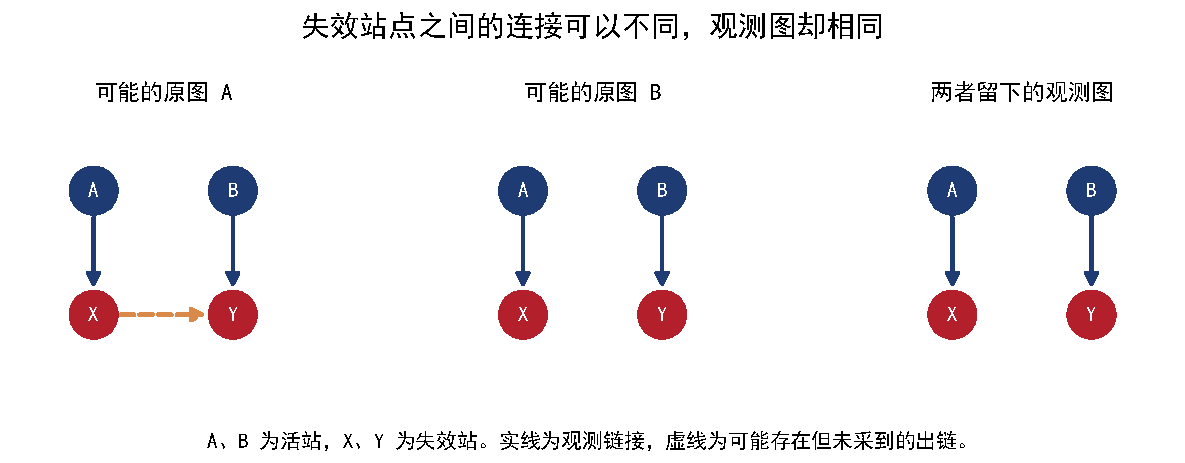
\includegraphics[width=0.80\linewidth]{fig11_missing_outlinks.pdf}
\caption{两张可能的原图经过出链遮蔽后留下相同的观测图。图中节点和连边仅用于解释观测机制。}
\end{figure}

D3 在控制抓取 URL 数量后，入度系数检验的 \(p\) 值为 0.4727，加入入度的交叉验证 AUC 增量为 0.0068。这说明入度对快照内失效标签的增量判别作用有限。检验能否预测未来失效，需要同站点在后续时点的状态和此前可用的预测特征。

\section{讨论与结论}

第一，无向二值图上的韧性结果适用于结构连通性。有向全图约 44.55\% 的有序点对可达，实际导航研究还需页面级出链。

第二，E5 的差异对抽样基线敏感。匹配使用快照中的分箱入度，层内仍可能有差异。故障对真实网络的影响需要用故障前后的观测数据检验。

第三，模板关联应按签名、邻接和样本分别报告。风险四象限的标签随度量口径改变，适用于比较群体情景。具体口径见方法手册。

这份子域图支持结构韧性比较。要进一步判断失效是否聚集，优先补充页面级出链和重复抓取。

\section*{数据与复现}

数据与原有产出见 \url{https://github.com/ge-shuai/CSA_HW}（基线 \texttt{51ccc5e}）。主证据来自 A4、D3、D4、E3 与 E5。E5 目录包含补充脚本、分层配额、600 次抽样及摘要表，新增两图可由 \texttt{render\_followup.py} 重建。

\enlargethispage{\baselineskip}
\begin{thebibliography}{9}
\bibitem{albert2000} Albert R., Jeong H., Barabási A.-L. Error and attack tolerance of complex networks. \emph{Nature}, 406, 378--382, 2000.
\bibitem{broder2000} Broder A., Kumar R., Maghoul F., et al. Graph structure in the Web. \emph{Computer Networks}, 33, 309--320, 2000.
\end{thebibliography}

\end{document}
